
A sanitizer is a kind of technique that checks certain runtime properties of the code (probe) that's inserted by the compiler. People usually use a sanitizer to ensure program correctness or enforce security policies. To give you an idea of how a sanitizer works, let's use one of the most popular sanitizers in Clang as an example – the address sanitizer.

\subsubsubsection{12.2.1\hspace{0.2cm}An example of using an address sanitizer}

Let's assume we have some simple C code, such as the following:

\begin{lstlisting}[style=styleCXX]
int main(int argc, char **argv) {
	int buffer[3];
	for (int i = 1; i < argc; ++i)
		buffer[i-1] = atoi(argv[i]);
		
	for (int i = 1; i < argc; ++i)
		printf("%d ", buffer[i-1]);
	printf("\n");
	return 0;
}
\end{lstlisting}

The preceding code converted the command-line arguments into integers and stored them in a buffer of size 3. Then, we printed them out.

You should be able to easily spot an outstanding problem: the value of argc can be arbitrarily big when it's larger than 3 – the size of buffer. Here, we are storing the value in an invalid memory location. However, when we compile this code, the compiler will say nothing. Here is an example:

\begin{tcblisting}{commandshell={}}
$ clang -Wall buffer_overflow.c -o buffer_overflow
$ # No error or warning
\end{tcblisting}

In the preceding command, even if we enable all the compiler warnings via the -Wall flag, clang won't complain about the potential bug.

If we try to execute the buffer\_overflow program, the program will crash at some time point after we pass more than three command-line arguments to it; for example:

\begin{tcblisting}{commandshell={}}
$ ./buffer_overflow 1 2 3
1 2 3
$ ./buffer_overflow 1 2 3 4
Segmentation fault (core dumped)
$
\end{tcblisting}

What's worse, the number of command-line arguments to crash buffer\_overflow actually varies from machine to machine. This makes it even more difficult to debug if the example shown here were a real-world bug. To summarize, the problem we're encountering here is caused by the fact that buffer\_overflow only goes rogue on some inputs and the compiler failed to catch the problem. 

Now, let's try to use an address sanitizer to catch this bug. The following command asks clang to compile the same code with an address sanitizer:


\begin{tcblisting}{commandshell={}}
$ clang -fsanitize=address buffer_overflow.c -o san_buffer_overflow
\end{tcblisting}

Let's execute the program again. Here is the output:

\begin{tcblisting}{commandshell={}}
$ ./san_buffer_overflow 1 2 3
1 2 3
$ ./san_buffer_overflow 1 2 3 4
==============================================================
===
==137791==ERROR: AddressSanitizer: stack-buffer-overflow on
address 0x7ffea06bccac at pc 0x0000004f96df bp 0x7ffea06bcc70…
WRITE of size 4 at 0x7ffea06bccac thread T0
…
  This frame has 1 object(s):
    [32, 44) 'buffer' <== Memory access at offset 44 overflows this variable
…
==137791==ABORTING
$
\end{tcblisting}

Instead of just crashing, the address sanitizer gave us many details about the issue that was raised at runtime: the sanitizer told us that it detected a buffer overflow on the stack, which might be the buffer variable.

These messages were extremely useful. Imagine that you are working on a much more complicated software project. When a strange memory bug occurs, rather than just crash or silently change the program's logic, the address sanitizer can point out the problematic area – with high accuracy – right away.

To go a little deeper into its mechanisms, the following diagram illustrates how the address sanitizer detects the buffer overflow:

\hspace*{\fill} \\ %插入空行
\begin{center}
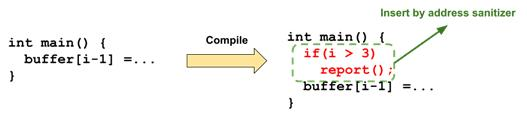
\includegraphics[width=0.9\textwidth]{content/3/chapter12/images/1.png}\\
Figure 12.1 – Instrumentation code inserted by the address sanitizer
\end{center}

Here, we can see that the address sanitizer is effectively inserting a boundary check into the array index that's used for accessing buffer. With this extra check – which will be executed at runtime – the target program can bail out with error details before violating the memory access. More generally speaking, during the compilation, a sanitizer inserts some instrumentation code (into the target program) that will eventually be executed at runtime to check or guard certain properties.

\begin{tcolorbox}[colback=blue!5!white,colframe=blue!75!black, fonttitle=\bfseries,title=Detecting overflow using an address sanitizer]	
\hspace*{0.7cm}The preceding diagram shows a simplified version of how an address sanitizer works. In reality, the address sanitizer will leverage multiple strategies to monitor memory access in a program. For example, an address sanitizer can use a special memory allocator that allocates memory with traps put at the invalid memory region.
\end{tcolorbox}

While an address sanitizer is specialized in catching illegal memory access, a ThreadSanitizer can be used to catch data race conditions; that is, invalid access from multiple threads on the same chunk of data. Some other examples of sanitizers in Clang are the LeakSanitizer, which is used for detecting sensitive data such as passwords being leaked, and MemorySanitizer, which is used for detecting reads to uninitialized memory.

Of course, there are some downsides to using sanitizers. The most prominent problem is the performance impact: using a thread sanitizer (in Clang) as an example, programs that are compiled with one are 5~15 times slower than the original version. Also, since sanitizers insert extra code into the program, it might hinder some optimization opportunities, or even affect the original program's logic! In other words, it is a trade-off between the robustness and performance of the target program.

With that, you've learned about the high-level idea of a sanitizer. Let's try to create a real one by ourselves to understand how Clang and LLVM implement a sanitizer. The following section contains more code than any of the examples in previous chapters, not to mention the changes are spread across different subprojects in LLVM. To focus on the most important knowledge, we won't go into the details of some supporting code – for example, changes that are made to CMake build scripts. Instead, we will go through them by providing a brief introduction and pointing out where you can find it in this book's GitHub repository.

Let's start by providing an overview of the project we are going to create.


\subsubsubsection{12.2.2\hspace{0.2cm}Creating a loop counter sanitizer}

To (slightly) simplify our task, the sanitizer we are going to create – a loop counter sanitizer, or LPCSan for short – looks just like a sanitizer except that it is not checking any serious program properties. Instead, we want to use it to print out the real, concrete trip count – the number of iterations – of a loop, which is only available during runtime.

For example, let's assume we have the following input code:

\begin{lstlisting}[style=styleCXX]
void foo(int S, int E, int ST, int *a) {
	for (int i = S; i < E; i += ST) {
		a[i] = a[i + 1];
	}
}
int main(int argc, char **argv) {
	int start = atoi(argv[1]),
	    end = atoi(argv[2]),
	    step = atoi(argv[3]);
	int a[100];
	foo(start, end, step, a);
	return 0;
}
\end{lstlisting}

We can compile it with a LPCSan using the following command:

\begin{tcblisting}{commandshell={}}
$ clang -O1 -fsanitize=loop-counter test_lpcsan.c -o test_lpcsan
\end{tcblisting}

Note that compiling with optimization greater than -O0 is necessary; we will explain why later.

When we execute test\_lpcsan (with some command-line argument), we can print out the precise trip count of the loop in the foo function. For example, look at the following code:

\begin{tcblisting}{commandshell={}}
$ ./test_lpcsan 0 100 1
==143813==INFO: Found a loop with trip count 100
$ ./test_lpcsan 0 50 2
==143814==INFO: Found a loop with trip count 25
$
\end{tcblisting}

The message highlighted in the preceding code was printed by our sanitizer code. 

Now, let's dive into the steps for creating the LPCSan. We will divide this tutorial into three parts:

\begin{itemize}
\item Developing an IR transformation
\item Adding Compiler-RT components
\item Adding the LPCSan to Clang
\end{itemize}

We will start with the IR transformation part of this sanitizer.


\hspace*{\fill} \\ %插入空行
\noindent
\textbf{Developing an IR transformation}

Previously, we learned that an address sanitizer – or just a sanitizer in general – usually inserts code into the target program to check certain runtime properties or collect data. In Chapter 9, Working with PassManager and AnalysisManager, and Chapter 10, Processing LLVM IR, we learned how to modify/transform LLVM IR, including inserting new code into it, so this seems to be a good starting point for crafting our LPCSan. 

In this section, we are going to develop an LLVM pass called LoopCounterSanitizer that inserts special function calls to collect the exact trip count of every loop in Module. Here are the detailed steps:

\begin{enumerate}
\item First, let's create two files: LoopCounterSanitizer.cpp under the llvm/lib/Transforms/Instrumentation folder and its corresponding header file inside the llvm/include/llvm/Transforms/Instrumentation folder. Inside the header file, we will place the declaration of this pass, as shown here:

\begin{lstlisting}[style=styleCXX]
struct LoopCounterSanitizer
: public PassInfoMixin<LoopCounterSanitizer> {
	PreservedAnalyses run(Loop&, LoopAnalysisManager&,
						  LoopStandardAnalysisResults&,
						  LPMUpdater&);
private:
	// Sanitizer functions
	FunctionCallee LPCSetStartFn, LPCAtEndFn;
	void initializeSanitizerFuncs(Loop&);
};
\end{lstlisting}

The preceding code shows the typical loop pass structure we saw in Chapter 10, Processing LLVM IR. The only notable changes are the LPCSetStartFn and LPCAtEndFn memory variables – they will store the Function instances that collect loop trip counts (FunctionCallee is a thin wrapper around Function that provides additional function signature information).

\item Finally, in LoopCounterSanitizer.cpp, we are placing the skeleton code for our pass, as shown here:

\begin{lstlisting}[style=styleCXX]
PreservedAnalyses
LoopCounterSanitizer::run(Loop &LP, LoopAnalysisManager
&LAM, LoopStandardAnalysisResults &LSR, LPMUpdater &U) {
	initializeSanitizerFuncs(LP);
	return PreservedAnalyses::all();
}
\end{lstlisting}

The initializeSanitizerFuncs method in the preceding code will populate LPCSetStartFn and LPCAtEndFn. Before we go into the details of initializeSanitizerFuncs, let's talk more about LPCSetStartFn and LPCAtEndFn.

\item To figure out the exact trip count, the Function instance stored in LPCSetStartFn will be used to collect the initial induction variable value of a loop. On the other hand, the Function instance stored in LPCAtEndFn will be used to collect the final induction variable value and the step value of the loop. To give you a concrete idea of how these two Function instances work together, let's assume we have the following pseudocode as our input program:

\begin{lstlisting}[style=styleCXX]
void foo(int S, int E, int ST) {
	for (int i = S; i < E; i += ST) {
		…
	}
}
\end{lstlisting}

In the preceding code, the S, E, and ST variables represent the initial, final, and step values of a loop, respectively. The goal of the  LoopCounterSanitizer pass is to insert LPCSetStartFn and LPCAtEndFn in the following way:

\begin{lstlisting}[style=styleCXX]
void foo(int S, int E, int ST) {
	for (int i = S; i < E; i += ST) {
		lpc_set_start(S);
		…
		lpc_at_end(E, ST);
	}
}
\end{lstlisting}

lpc\_set\_start and lpc\_at\_end in the preceding code are Function instances that are stored in LPCSetStartFn and LPCAtEndFn, respectively. Here is one of the possible (pseudo) implementations of these two functions:

\begin{lstlisting}[style=styleCXX]
static int CurrentStartVal = 0;
void lpc_set_start(int start) {
	CurrentStartVal = start;
}
void lpc_at_end(int end, int step) {
	int trip_count = (end – CurrentStartVal) / step;
	printf("Found a loop with trip count %d\n",
	trip_count);
}
\end{lstlisting}

Now that we know the roles of LPCSetStartFn and LPCAtEndFn, it's time to take a look at how initializeSanitizerFuncs initializes them.

\item Here is the code inside initializeSanitizerFuncs:

\begin{lstlisting}[style=styleCXX]
void LoopCounterSanitizer::initializeSanitizerFuncs(Loop
&LP) {
	Module &M = *LP.getHeader()->getModule();
	auto &Ctx = M.getContext();
	Type *VoidTy = Type::getVoidTy(Ctx),
	     *ArgTy = Type::getInt32Ty(Ctx);
	LPCSetStartFn
	  = M.getOrInsertFunction("__lpcsan_set_loop_start",
	                          VoidTy, ArgTy);
	LPCAtEndFn = M.getOrInsertFunction("__lpcsan_at_loop_
	  end", VoidTy, ArgTy, ArgTy);
}
\end{lstlisting}

The previous code is basically fetching two functions, \_\_lpcsan\_set\_loop\_ start and \_\_lpcsan\_at\_loop\_end, from the module and storing their Function instances in LPCSetStartFn and LPCAtEndFn, respectively.

The Module::getOrInsertFunction method either grabs the Function instance of the given function name from the module or creates one if it doesn't exist. If it's a newly created instance, it has an empty function body; in other words, it only has a function declaration.

It is also worth noting that the second argument of Module::getOrInsertFunction is the return type of the Function inquiry. The rest (the arguments for getOrInsertFunction) represent the argument types of that Function.

With LPCSetStartFn and LPCAtEndFn set up, let's see how we can insert them into the right place in IR.

\item Recall that in Chapter 10, Processing LLVM IR, we learned about several utility classes for working with Loop. One of them – LoopBounds – can give us the boundary of a Loop. We can do this by including the start, end, and step values of an induction variable, which is exactly the information we are looking for. Here is the code that tries to retrieve a LoopBounds instance:

\begin{lstlisting}[style=styleCXX]
PreservedAnalyses
LoopCounterSanitizer::run(Loop &LP, LoopAnalysisManager
&LAM, LoopStandardAnalysisResults &LSR, LPMUpdater &U) {
	initializeSanitizerFuncs(LP);
	ScalarEvolution &SE = LSR.SE;
	
	using LoopBounds = typename Loop::LoopBounds;
	auto MaybeLB = LP.getBounds(SE);
	if (!MaybeLB) {
		errs() << "WARNING: Failed to get loop bounds\n";
		return PreservedAnalyses::all();
	}
	LoopBounds &LB = *MaybeLB;
	…
	Value *StartVal = &LB.getInitialIVValue(),
		  *EndVal = &LB.getFinalIVValue(),
		  *StepVal = LB.getStepValue();
}
\end{lstlisting}

Loop::getBounds from the preceding code returned an Optional<LoopBounds> instance. The Optional<T> class is a useful container that either stores an instance of the T type or is empty. You can think of it as a replacement for the null pointer: usually, people use T* to represent a computation result where a null pointer means an empty value. However, this has the risk of dereferencing a null pointer if the programmer forgets to check the pointer first. The Optional<T> class doesn't have this problem.

With a LoopBounds instance, we can retrieve the induction variable's range and store it in the StartVal, EndVal, and StepVal variables.

\item StartVal is the Value instance to be collected by \_\_lpcsan\_set\_loop\_ start, whereas \_\_lpcsan\_at\_loop\_end is going to collect EndVal and StepVal at runtime. Now, the question is, where should we insert function calls to \_\_lpcsan\_set\_loop\_start and \_\_lpcsan\_at\_loop\_end to correctly collect those values?

The rule of thumb is that we need to insert those function calls after the definition of those values. While we can find the exact locations where those values were defined, let's try to simplify the problem by inserting instrumentation function calls at some fixed locations – locations where our target values are always available.

For \_\_lpcsan\_set\_loop\_start, we are inserting it at the end of the loop header block, because the initial induction variable value will never be defined after this block. Here is the code:

\begin{lstlisting}[style=styleCXX]
// Inside LoopCounterSanitizer::run …
…
BasicBlock *Header = LP.getHeader();
Instruction *LastInst = Header->getTerminator();
IRBuilder<> Builder(LastInst);
Type *ArgTy = LPCSetStartFn.getFunctionType()-
>getParamType(0);
if (StartVal->getType() != ArgTy) {
	// cast to argument type first
	StartVal = Builder.CreateIntCast(StartVal, ArgTy,
	true);
}
Builder.CreateCall(LPCSetStartFn, {StartVal});
…
\end{lstlisting}

In the preceding code, we used getTerminator to get the last Instruction from the header block. Then, we used IRBuilder<> – with the last instruction as the insertion point – to insert new Instruction instances.

Before we can pass StartVal as an argument to the new \_\_lpcsan\_set\_loop\_ start function call, we need to convert its IR type (represented by the Type class) into a compatible one. IRBuilder::CreateInstCast is a handy utility that automatically generates either an instruction to extend the integer bit width or an instruction to truncate the bit width, depending on the given Value and Type instances.

Finally, we can create a function call to \_\_lpcsan\_set\_loop\_start via IRBuilder::CreateCall, with StartVal as the function call argument.

\item For \_\_lpcsan\_at\_loop\_end, we are using the same trick to collect the runtime values of EndVal and StepVal. Here is the code:

\begin{lstlisting}[style=styleCXX]
BasicBlock *ExitBlock = LP.getExitBlock();
Instruction *FirstInst = ExitBlock->getFirstNonPHI();
IRBuilder<> Builder(FirstInst);
FunctionType *LPCAtEndTy = LPCAtEndFn.getFunctionType();
Type *EndArgTy = LPCAtEndTy->getParamType(0),
     *StepArgTy = LPCAtEndTy->getParamType(1);

if (EndVal->getType() != EndArgTy)
	EndVal = Builder.CreateIntCast(EndVal, EndArgTy, true);
if (StepVal->getType() != StepArgTy)
	StepVal = Builder.CreateIntCast(StepVal, StepArgTy,
		true);
		
Builder.CreateCall(LPCAtEndFn, {EndVal, StepVal});
\end{lstlisting}

Different from the previous step, we are inserting the function call to \_\_lpcsan\_at\_loop\_end at the beginning of the exit block. This is because we can always expect the end value and the step value of the induction variable being defined before we leave the loop.

These are all the implementation details for the LoopCounterSanitizer pass.

\item Before we wrap up this section, we need to edit a few more files to make sure everything works. Please look at the Changes-LLVM.diff file in the sample code folder for this chapter. Here is the summary of the changes that were made in other supporting files:

\begin{enumerate}[label=\roman*.]
\item Changes in llvm/lib/Transforms/Instrumentation/CMakeLists.txt: Add our new pass source file to the build.
\item Changes in llvm/lib/Passes/PassRegistry.def: Add our pass to the list of available passes so that we can test it using our old friend opt.
\end{enumerate}

\end{enumerate}

With that, we've finally finished making all the necessary modifications to the LLVM part.

Before we move on to the next section, let's test our newly created LoopCounterSanitizer pass. We are going to be using the same C code we saw earlier in this section. Here is the function that contains the loop we want to instrument:

\begin{lstlisting}[style=styleCXX]
void foo(int S, int E, int ST, int *a) {
	for (int i = S; i < E; i += ST) {
		a[i] = a[i + 1];
	}
}
\end{lstlisting}

Note that although we didn't explicitly check the loop form in our pass, some of the APIs that were used in the pass actually required the loop to be rotated, so please generate the LLVM IR code with an O1 optimization level to make sure the loop rotation's Pass has kicked in:

Here is the simplified LLVM IR for the foo function:

\begin{lstlisting}[style=styleCXX]
define void @foo(i32 %S, i32 %E, i32 %ST, i32* %a) {
	%cmp9 = icmp slt i32 %S, %E
	br i1 %cmp9, label %for.body.preheader, label %for.cond.
	cleanup
for.body.preheader:
	%0 = sext i32 %S to i64
	%1 = sext i32 %ST to i64
	%2 = sext i32 %E to i64
	br label %for.body
	…
for.body:
	%indvars.iv = phi i64 [ %0, %for.body.preheader ], [
	%indvars.iv.next, %for.body ]
	…
	%indvars.iv.next = add i64 %indvars.iv, %1
	%cmp = icmp slt i64 %indvars.iv.next, %2
	br i1 %cmp, label %for.body, label %for.cond.cleanup
}
\end{lstlisting}

The highlighted labels are the preheader and loop body blocks for this loop. Since this loop has been rotated, the for.body block is both the header, latch, and exiting block for this loop.

Now, let's transform this IR with opt using the following command:

\begin{tcblisting}{commandshell={}}
$ opt -S –passes="loop(lpcsan)" input.ll -o -
\end{tcblisting}

In the –passes command-line option, we asked opt to run our LoopCounterSanitizer pass (with the name lpcsan, which is registered in the PassRegistry.def file). The enclosing loop(…) string is simply telling opt that lpcsan is a loop pass (you can actually omit this decoration since opt can find the right pass most of the time).

Here is the simplified result:

\begin{lstlisting}[style=styleCXX]
declare void @__lpcsan_set_loop_start(i32)
declare void @__lpcsan_at_loop_end(i32, i32)

define void @foo(i32 %S, i32 %E, i32* %a) {
	%cmp8 = icmp slt i32 %S, %E
	br i1 %cmp8, label %for.body.preheader, label %for.cond.
cleanup
	
for.body.preheader:
	%0 = sext i32 %S to i64
	%wide.trip.count = sext i32 %E to i64
	br label %for.body
	
for.cond.cleanup.loopexit:
	%1 = trunc i64 %wide.trip.count to i32
	call void @__lpcsan_at_loop_end(i32 %1, i32 1)
	br label %for.cond.cleanup
	
for.body:
	…
	%3 = trunc i64 %0 to i32
	call void @__lpcsan_set_loop_start(i32 %3)
	br i1 %exitcond.not, label %for.cond.cleanup.loopexit, label
	  %for.body
}
\end{lstlisting}

As you can see, \_\_lpcsan\_set\_loop\_start and \_\_lpcsan\_at\_loop\_end have been correctly inserted into the header block and exit block, respectively. They are also collecting the desired values related to the loop trip count.

Now, the biggest question is: where are the function bodies for \_\_lpcsan\_set\_loop\_start and \_\_lpcsan\_at\_loop\_end? Both only have declarations in the preceding IR code.

In the next section, we will use Compiler-RT to answer this question.

\hspace*{\fill} \\ %插入空行
\noindent
\textbf{Adding the Compiler-RT component}

The name Compiler-RT stands for Compiler RunTime. The usage of runtime is a little ambiguous here because too many things can be called a runtime in a normal compilation pipeline. But the truth is that Compiler-RT does contain a wide range of libraries for completely different tasks. What these libraries have in common is that they provide supplement code for the target program to implement enhancement features or functionalities that were otherwise absent. It is important to remember that Compiler-RT libraries are NOT used for building a compiler or related tool – they should be linked with the program we are compiling.

One of the most used features in Compiler-RT is the builtin function. As you might have heard, more and more computer architectures nowadays support vector operation natively. That is, you can process multiple data elements at the same time with the support from hardware. Here is some example code, written in C, that uses vector operations:

\begin{lstlisting}[style=styleCXX]
typedef int v4si __attribute__((__vector_size__(16)));
v4si v1 = (v4si){1, 2, 3, 4};
v4si v2 = (v4si){5, 6, 7, 8};
v4si v3 = v1 + v2; // = {6, 8, 10, 12}
\end{lstlisting}


The preceding code used a non-standardized (currently, you can only use this syntax in Clang and GCC) C/C++ vector extension to declare two vectors, v1 and v2, before adding them to yield a third one.

On X86-64 platforms, this code will be compiled to use one of the vector instruction sets, such as SSE or AVX. On the ARM platform, the resulting binary might be using the NEON vector instruction set. But what if your target platform does NOT have a vector instruction set? The most obvious solution would be "synthesizing" these unsupported operations with the available instructions. For example, we should write a for-loop to replace vector summation in this case. More specifically, whenever we see a vector summation at compilation time, we replace it with a call to a function that contains the synthesis implementation using for-loop. The function body can be put anywhere, as long as it is eventually linked with the program. The following diagram illustrates this process:

\hspace*{\fill} \\ %插入空行
\begin{center}
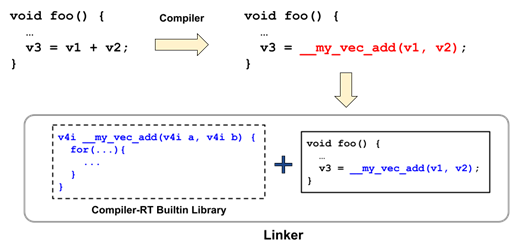
\includegraphics[width=0.9\textwidth]{content/3/chapter12/images/2.png}\\
Figure 12.2 – Workflow of the Compiler-RT builtin
\end{center}

As you may have noticed, the workflow shown here is similar to our requirement in the LPCSan: in the previous section, we developed an LLVM pass that inserted extra function calls to collect the loop trip count, but we still need to implement those collector functions. If we leverage the workflow shown in the preceding diagram, we can come up with a design, as shown in the following diagram:

\hspace*{\fill} \\ %插入空行
\begin{center}
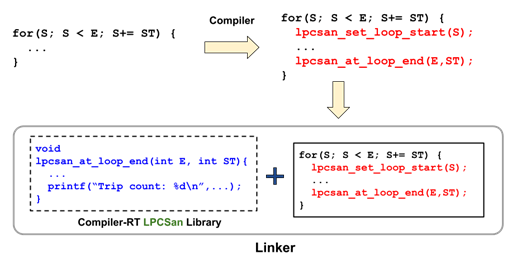
\includegraphics[width=0.9\textwidth]{content/3/chapter12/images/3.png}\\
Figure 12.3 – Workflow of the Compiler-RT LPCSan component
\end{center}

The previous diagram shows that the function bodies of \_\_lpcsan\_set\_loop\_start and \_\_lpcsan\_at\_loop\_end are put inside a Compiler-RT library that will eventually be linked with the final binary. Inside these two functions, we calculate the trip count using the input arguments and print the result. In the rest of this section, we'll show you how to create such a Compiler-RT library for the LPCSan. Let's get started:

\begin{itemize}
\item First, switch the folder to llvm-project/compiler-rt, the root of Compiler-RT. Inside this subproject, we must create a new folder called lib/lpcsan before we put a new lpcsan.cpp file inside it. Within this file, let's create the skeleton for our instrumentation functions. Here is the code:

\begin{lstlisting}[style=styleCXX]
#include "sanitizer_common/sanitizer_common.h"
#include "sanitizer_common/sanitizer_internal_defs.h"
using namespace __sanitizer;

extern "C" SANITIZER_INTERFACE_ATTRIBUTE
void __lpcsan_set_loop_start(s32 start){
	// TODO
}
extern "C" SANITIZER_INTERFACE_ATTRIBUTE
void __lpcsan_at_loop_end(s32 end, s32 step){
	// TODO
}
\end{lstlisting}

There are two things worth noting here: first, use the primitive data types provided by Compiler-RT. For example, in the preceding code, we used s32 – available under the \_\_sanitizer namespace – for a signed 32-bit integer rather than the normal int. The rationale behind this is that we might need to build Compiler-RT libraries for different hardware architectures or platforms, and the width of int might not be 32 bits on some of them.

Second, although we are using C++ to implement our instrumentation functions, we need to expose them as C functions because C functions have a more stable Application Binary Interface (ABI). Therefore, please make sure to add extern "C" to functions you want to export. The SANITIZER\_INTERFACE\_ATTRIBUTE macro also ensures that the function will be exposed at the library interface correctly, so please add this as well.

\item Next, we will add the necessary code to these two functions. Here is how we do this:

\begin{lstlisting}[style=styleCXX]
static s32 CurLoopStart = 0;
extern "C" SANITIZER_INTERFACE_ATTRIBUTE
void __lpcsan_set_loop_start(s32 start){
	CurLoopStart = start;
}
extern "C" SANITIZER_INTERFACE_ATTRIBUTE
void __lpcsan_at_loop_end(s32 end, s32 step){
	s32 trip_count = (end - CurLoopStart) / step;
	s32 abs_trip_count
	  = trip_count >= 0? trip_count : -trip_count;
	Report("INFO: Found a loop with "
	       "trip count %d\n", abs_trip_count);
}
\end{lstlisting}

The implementation we used here is pretty straightforward: CurLoopStart is a global variable that memorizes the initial induction variable value of the current loop. This is updated by \_\_lpcsan\_set\_loop\_start.

Recall that when a loop is complete, \_\_lpcsan\_at\_loop\_end will be invoked. When that happens, we use the value stored in CurLoopStart and the end and step arguments to calculate the exact trip count of the current loop, before printing the result.

\item Now that we have implemented the core logic, it's time to build this library. Inside the lib/lpcsan folder, create a new CMakeLists.txt file and insert the following code:

\begin{lstlisting}[style=styleCMake]
…
set(LPCSAN_RTL_SOURCES
	lpcsan.cpp)
add_compiler_rt_component(lpcsan)

foreach(arch ${LPCSAN_SUPPORTED_ARCH})
	set(LPCSAN_CFLAGS ${LPCSAN_COMMON_CFLAGS})
	add_compiler_rt_runtime(clang_rt.lpcsan
		STATIC
		ARCHS ${arch}
		SOURCES ${LPCSAN_RTL_SOURCES}
				$<TARGET_OBJECTS:RTSanitizerCommon.${arch}>
				$<TARGET_OBJECTS:RTSanitizerCommonLibc.${arch}>
		ADDITIONAL_HEADERS ${LPCSAN_RTL_HEADERS}
		CFLAGS ${LPCSAN_CFLAGS}
		PARENT_TARGET lpcsan)
	…
endforeach()
\end{lstlisting}

In the preceding code, we are only showing the most important part of our CMakeLists.txt. Here are some highlights:


\begin{enumerate}[label=\roman*.]
\item Compiler-RT creates its own set of CMake macros/functions. Here, we are using two of them, add\_compiler\_rt\_component and add\_compiler\_rt\_runtime, to create a pseudo build target for the entire LPCSan and the real library build target, respectively.

\item Different from a conventional build target, if a sanitizer wants to use supporting/utility libraries in Compiler-RT – for example, RTSanitizerCommon in the preceding code – we usually link against their object files rather than their library files. More specifically, we can use the \$<TARGET\_OBJECTS:…> directive to import supporting/utility components as one of the input sources.

\item A sanitizer library can support multiple architectures and platforms. In Compiler-RT, we are enumerating all the supported architectures and creating a sanitizer library for each of them.

Again, the preceding snippet is just a small part of our build script. Please refer to our sample code folder for the complete CMakeLists.txt file.
\end{enumerate}

\item To successfully build the LPCSan, we still need to make some changes in Compiler-RT. The Base-CompilerRT.diff patch in the same code folder provides the rest of the changes that are necessary to build our sanitizer. Apply it to Compiler-RT's source tree. Here is the summary of this patch:

\begin{enumerate}[label=\roman*.]
\item Changes in compiler-rt/cmake/config-ix.cmake basically specify the supported architectures and operating systems of the LPCSan. The LPCSAN\_SUPPORTED\_ARCH CMake variable we saw in the previous snippet comes from here.

\item The entire compiler-rt/test/lpcsan folder is actually a placeholder. For some reason, having tests is a requirement for every sanitizer in Compiler-RT – which is different from LLVM. Therefore, we are putting an empty test folder here to pass this requirement that's being imposed by the build infrastructure.
\end{enumerate}

\end{itemize}

These are all the steps for producing a Compiler-RT component for our LPCSan.

To just build our LPCSan library, invoke the following command:

\begin{tcblisting}{commandshell={}}
$ ninja lpcsan
\end{tcblisting}

Unfortunately, we can't test this LPCSan library until we've modified the compilation pipeline in Clang. In the last part of this section, we are going to learn how to achieve this task.

\hspace*{\fill} \\ %插入空行
\noindent
\textbf{Adding the LPCSan to Clang}

In the previous section, we learned how Compiler-RT libraries provide supplement functionalities to the target program or assist with special instrumentation, such as the sanitizer we just created. In this section, we are going to put everything together so that we can use our LPCSan simply by passing the -fsanitize=loop-counter flag to clang.

Recall that in Figure 12.3, Compiler-RT libraries need to be linked with the program we are compiling. Also, recall that in order to insert the instrumentation code into the target program, we must run our LoopCounterSanitizer pass. In this section, we are going to modify the compilation pipeline in Clang so that it runs our LLVM pass at a certain time and sets up the correct configuration for our Compiler-RT library. More specifically, the following diagram shows the tasks that each component needs to complete to run our LPCSan:

\hspace*{\fill} \\ %插入空行
\begin{center}
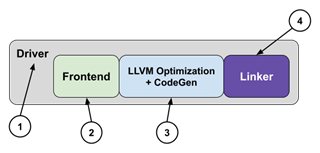
\includegraphics[width=0.9\textwidth]{content/3/chapter12/images/4.png}\\
Figure 12.4 – Tasks for each component in the pipeline
\end{center}

Here are the descriptions for each of the numbers (enclosed in circles) in the preceding diagram:

\begin{itemize}
\item The driver needs to recognize the -fsanitize=loop-counter flag.
\item When the frontend is about to generate LLVM IR from an Abstract Syntax Tree (AST), it needs to correctly configure the LLVM pass pipeline so that it includes the LoopCounterSanitizer pass.
\item The LLVM pass pipeline needs to run our LoopCounterSanitizer (we don't need to worry about this task if the previous task is done correctly).
\item The linker needs to link our Compiler-RT library to the target program.
\end{itemize}

Although this workflow looks a little scary, don't be overwhelmed by the prospective workload – Clang can actually do most of these tasks for you, as long as you provide sufficient information. In the rest of this section, we'll show you how to implement the tasks shown in the preceding diagram to fully integrate our LPCSan into the Clang compilation pipeline (the following tutorial works inside the llvm-project/clang folder). Let's get started:

\begin{enumerate}
\item First, we must modify include/clang/Basic/Sanitizers.def to add our sanitizer:

\begin{lstlisting}[style=styleCXX]
…
// Shadow Call Stack
SANITIZER("shadow-call-stack", ShadowCallStack)

// Loop Counter Sanitizer
SANITIZER("loop-counter", LoopCounter)
…
\end{lstlisting}

This effectively adds a new enum value, LoopCounter, to the SanitizerKind class.

It turns out that the driver will parse the -fsanitize command-line option and automatically translate loop-counter into SanitizerKind::LoopCounter based on the information we provided in Sanitizers.def.

\item Next, let's work on the driver part. Open include/clang/Driver/SanitizerArgs.h and add a new utility method, needsLpcsanRt, to the SanitizerArgs class. Here is the code:

\begin{lstlisting}[style=styleCXX]
bool needsLsanRt() const {…}
bool needsLpcsanRt() const {
	return Sanitizers.has(SanitizerKind::LoopCounter);
}
\end{lstlisting}

The utility method we created here can be used by other places in the driver to check if our sanitizer needs a Compiler-RT component.

\item Now, let's navigate to the lib/Driver/ToolChains/CommonArgs.cpp file. Here, we're adding a few lines to the collectSanitizerRuntimes function. Here is the code:

\begin{lstlisting}[style=styleCXX]
…
if (SanArgs.needsLsanRt() && SanArgs.linkRuntimes())
	StaticRuntimes.push_back("lsan");
if (SanArgs.needsLpcsanRt() && SanArgs.linkRuntimes())
	StaticRuntimes.push_back("lpcsan");
…
\end{lstlisting}

The preceding snippet effectively makes the linker link the correct Compiler-RT library to the target binary.

\item The last change we will make to the driver is in lib/Driver/ToolChains/Linux.cpp. Here, we add the following lines to the Linux::getSupportedSanitizers method:

\begin{lstlisting}[style=styleCXX]
SanitizerMask Res = ToolChain::getSupportedSanitizers();
…
Res |= SanitizerKind::LoopCounter;
…
\end{lstlisting}

The previous code is essentially telling the driver that we support the LPCSan in the current toolchain – the toolchain for Linux. Note that to simplify our example, we are only supporting the LPCSan in Linux. If you want to support this custom sanitizer in other platforms and architectures, modify the other toolchain implementations. Please refer to Chapter 8, Working with Compiler Flags and Toolchains, for more details if needed.


\item Finally, we are going to insert our LoopCounterSanitizer pass into the LLVM
pass pipeline. Open lib/CodeGen/BackendUtil.cpp and add the following
lines to the addSanitizers function:

\begin{lstlisting}[style=styleCXX]
…
// `PB` has the type of `PassBuilder`
PB.registerOptimizerLastEPCallback(
[&](ModulePassManager &MPM,
PassBuilder::OptimizationLevel Level) {
	…
	if (LangOpts.Sanitize.has(SanitizerKind::LoopCounter))
	{
		auto FA
		=
		createFunctionToLoopPassAdaptor(LoopCounterSanitizer());
		MPM.addPass(
		createModuleToFunctionPassAdaptor(std::move(FA)));
	}
});
…
\end{lstlisting}

The enclosing folder for this file, CodeGen, is a place where the Clang and LLVM libraries meet. Therefore, we will see several LLVM APIs appear in this place. There are primarily two tasks for this CodeGen component:

\begin{enumerate}[label=\alph*.]
\item Converting the Clang AST into its equivalent LLVM IR module
\item Constructing an LLVM pass pipeline to optimize the IR and generate machine code
\end{enumerate}

The previous snippet was trying to customize the second task – that is, customizing the LLVM Pass pipeline. The specific function – addSanitizers – we are modifying here is responsible for putting sanitizer passes into the pass pipeline. To have a better understanding of this code, let's focus on two of its components:

\begin{enumerate}[label=\roman*.]
\item PassBuilder: This class provides predefined pass pipeline configurations for each optimization level – that is, the O0 ~ O3 notations (as well as Os and Oz for size optimization) we are familiar with. In addition to these predefined layouts, developers are free to customize the pipeline by leveraging the extension point (EP).

An EP is a certain position in the (predefined) pass pipeline where you can insert new passes. Currently, PassBuilder supports several EPs, such as at the beginning of the pipeline, at the end of the pipeline, or at the end of the vectorization process, to name a few. An example of using EP can be found in the preceding code, where we used the PassBuilder::registerOptimizerLastEPCallback method and a lambda function to customize the EP located at the end of the Pass pipeline. The lambda function has two arguments: ModulePassManager – which represents the pass pipeline – and the current optimization level. Developers can use ModulePassManager::addPass to insert arbitrary LLVM passes into this EP.

\item ModulePassManager: This class represents a Pass pipeline – or, more
specifically, the pipeline for Module. There are, of course, other PassManager
classes for different IR units, such as FunctionPassManager for Function.

In the preceding code, we were trying to use the ModulePassManager instance to insert our LoopCounterSanitizer pass whenever SanitizerKind::LoopCounter was one of the sanitizers that had been designated by the user. Since LoopCounterSanitizer is a loop pass rather than a module pass, we need to add some adaptors between the pass and PassManager. The createFunctionToLoopPassAdaptor and createModuleToFunctionPassAdaptor functions we were using here created a special instance that adapts a pass to a PassManager of a different IR unit.

This is all the program logic that supports our LPCSan in the Clang compilation
pipeline.
\end{enumerate}

\item Last but not least, we must make a small modification to the build system. Open the runtime/CMakeLists.txt file and change the following CMake variable:

\begin{lstlisting}[style=styleCMake]
…
set(COMPILER_RT_RUNTIMES fuzzer asan builtins … lpcsan)
foreach(runtime ${COMPILER_RT_RUNTIMES})
…
\end{lstlisting}
The change we made to COMPILER\_RT\_RUNTIMES effectively imports our LPCSan Compiler-RT libraries into the build.


\end{enumerate}

These are all the steps necessary to support the LPCSan in Clang. Now, we can finally use the LPCSan in the same way we showed you at the beginning of this section:

\begin{tcblisting}{commandshell={}}
$ clang -O1 -fsanitize=loop-counter input.c -o input
\end{tcblisting}

In this section, we learned how to create a sanitizer. A sanitizer is a useful tool for
capturing runtime behaviors without modifying the original program code. The ability
to create a sanitizer increases the flexibility for compiler developers to create custom
diagnosing tools tailored for their own use cases. Developing a sanitizer requires
comprehensive knowledge of Clang, LLVM, and Compiler-RT: creating a new LLVM
pass, making a new Compiler-RT component, and customizing the compilation pipeline
in Clang. You can use the content in this section, to reinforce what you've learned in
previous chapters of this book.

In the last section of this chapter, we are going to look at one more instrumentation technique: PGO.















